\documentclass{article}

\usepackage{pgfplots}
\usetikzlibrary{calc}
\pgfplotsset{compat=1.14}



\begin{document}

\def\printpoint#1{%
	\pgfplotsextra{
		\scope
		\pgftransformshift{#1}%
		\fill[red] circle (1pt);
		\node [pin={
			\pgfplotspointgetcoordinates{#1}%
			$(%
				\pgfmathprintnumber[fixed,precision=1]{\pgfkeysvalueof{/data point/x}},%
				\pgfmathprintnumber[fixed,precision=1]{\pgfkeysvalueof{/data point/y}})$%
			}]
			{};
		\endscope
	}%
}%

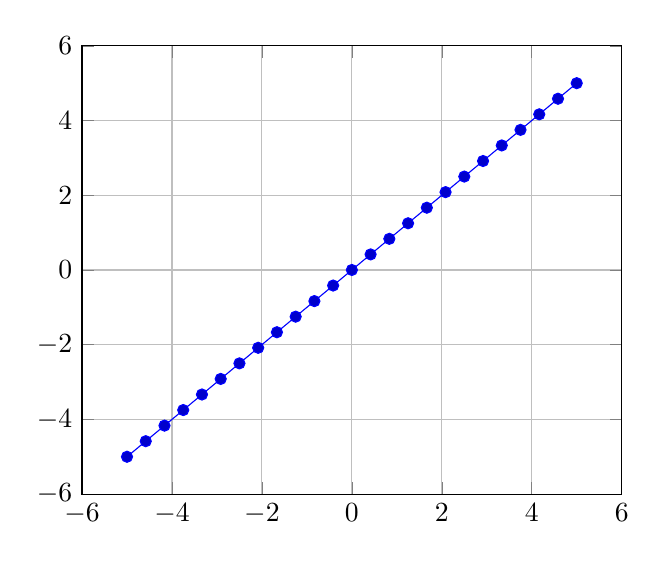
\begin{tikzpicture}
	\begin{axis}[clip=false,
		grid=both,
	]

	\addplot {x};

	\printpoint{\pgfpoint{150pt}{50pt}}%
	\printpoint{\pgfplotspointaxisxy{-2}{2}}
	\printpoint{\pgfplotspointaxisxy{-5}{-4}}

	\end{axis}
\end{tikzpicture}

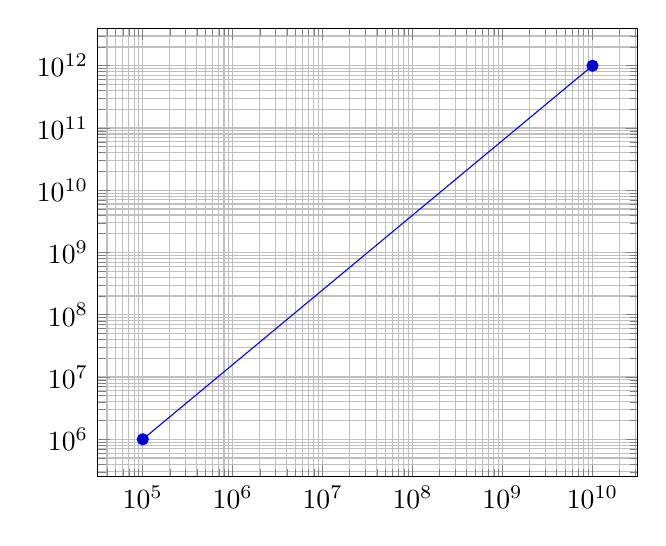
\begin{tikzpicture}
	\begin{loglogaxis}[
		clip=false,
		log basis x=10,
		log basis y=10,
		grid=both,
	]
	\addplot coordinates {(1e5,1e6) (1e10,1e12)};

	\printpoint{\pgfpoint{190pt}{180pt}}%
	\printpoint{\pgfplotspointaxisxy{1e6}{1e11}}

	\end{loglogaxis}
\end{tikzpicture}


\begin{tikzpicture}
\begin{axis}[
    height=6cm,
    width=14cm,
    %
    scale only axis=true,
    xlabel={Distance in mm},
    ylabel={Voltage in volt},
    ]
    \addplot [sharp plot, no marks, x=Wegnormiert] table {
    Wegnormiert abc
    0 -10
    130 10
    } coordinate [pos=0.5] (A) coordinate [pos=0.6] (B);
    \draw (A) -| (B);
    \filldraw let \p1= (A) in (\x1,\y1) circle [radius=1pt] node[pin={[pin distance=1.1cm]270:{{\pgfplotsconvertunittocoordinate{x}{\x1}\pgfmathprintnumber[fixed,precision=1]{\pgfmathresult}}}}] {};
    \filldraw let \p2= (B) in (\x2,\y2) circle (1pt) node[yshift=-0.5cm, pin=270:{{\pgfplotsconvertunittocoordinate{x}{\x2}\pgfmathprintnumber[fixed,precision=1]{\pgfmathresult}}}] {};

	\printpoint{\pgfpointanchor{A}{center}}
	\printpoint{\pgfpointanchor{B}{center}}
\end{axis}
\end{tikzpicture}
\end{document}
